% Matlab Implementation of Neural Field Model
% tex file of implementation document


\documentclass[a4paper, 12pt, english]{article}


% packages
\usepackage[english]{babel}
\usepackage{setspace}
\usepackage{amsmath}
\usepackage{graphicx}
\usepackage{float}
\usepackage{caption}


% graphic path
\graphicspath{{/Users/miao/Documents/Miao/Neurosciences/Projects/NeuralFieldModel/Figures/}}


% title of this manuscript
\title{Matlab Implementation of Neural Field Model}
\author{Miao Cao}
\date{1 July 2016}


\begin{document}
% set spacing of this document
\onehalfspacing

% title of the document
\begin{titlepage}\centering
\vspace*{\fill}
\maketitle
\vspace*{\fill}
\end{titlepage}

\tableofcontents

\newpage



% Introduction
\section{Introduction}
\paragraph{In order to implement and simulate Neural Field Model in Matlab, we break down
neural field model into several parts based mathematical equations and independently implement and test each part. The
following sections show the details of our implementation. Please always refer to
Freestone et al., 2011, NeuroImage for derivations, equations and details.}

\newpage




% Convolution of two Gaussians
\section{Convolution of Two Gaussian Basis Functions}

\paragraph{Analytically prove convolution of two Gaussians. In general, the
precision level of analytic simulation should be around $10^{-6}$.}

\paragraph{File (Matlab script): Convolution2DGaussians.m}

\subsection*{Matlab script description}

Appendix E (Freestone et al., 2011, NeuroImage), Equation (4) $\left(\phi_{i}\otimes\phi_{j}\right)(r)=(\frac{\pi\sigma_{i}^{2}\sigma_{j}^{2}}{\sigma_{i}^{2}+\sigma_{i}^{2}})^{\frac{n}{2}}\exp(-\frac{1}{\sigma_{i}^{2}+\sigma_{i}^{2}}r^{T}r)$.

\subparagraph{Section: Generate spatial data, create a $NPoints\times NPoints$ cortical surface and phi and psi Gaussian basis functions.\\}


\subsection{Parameters}



\subsection{Implementations}



\subsection{Results}
\begin{figure}[H]
\centering
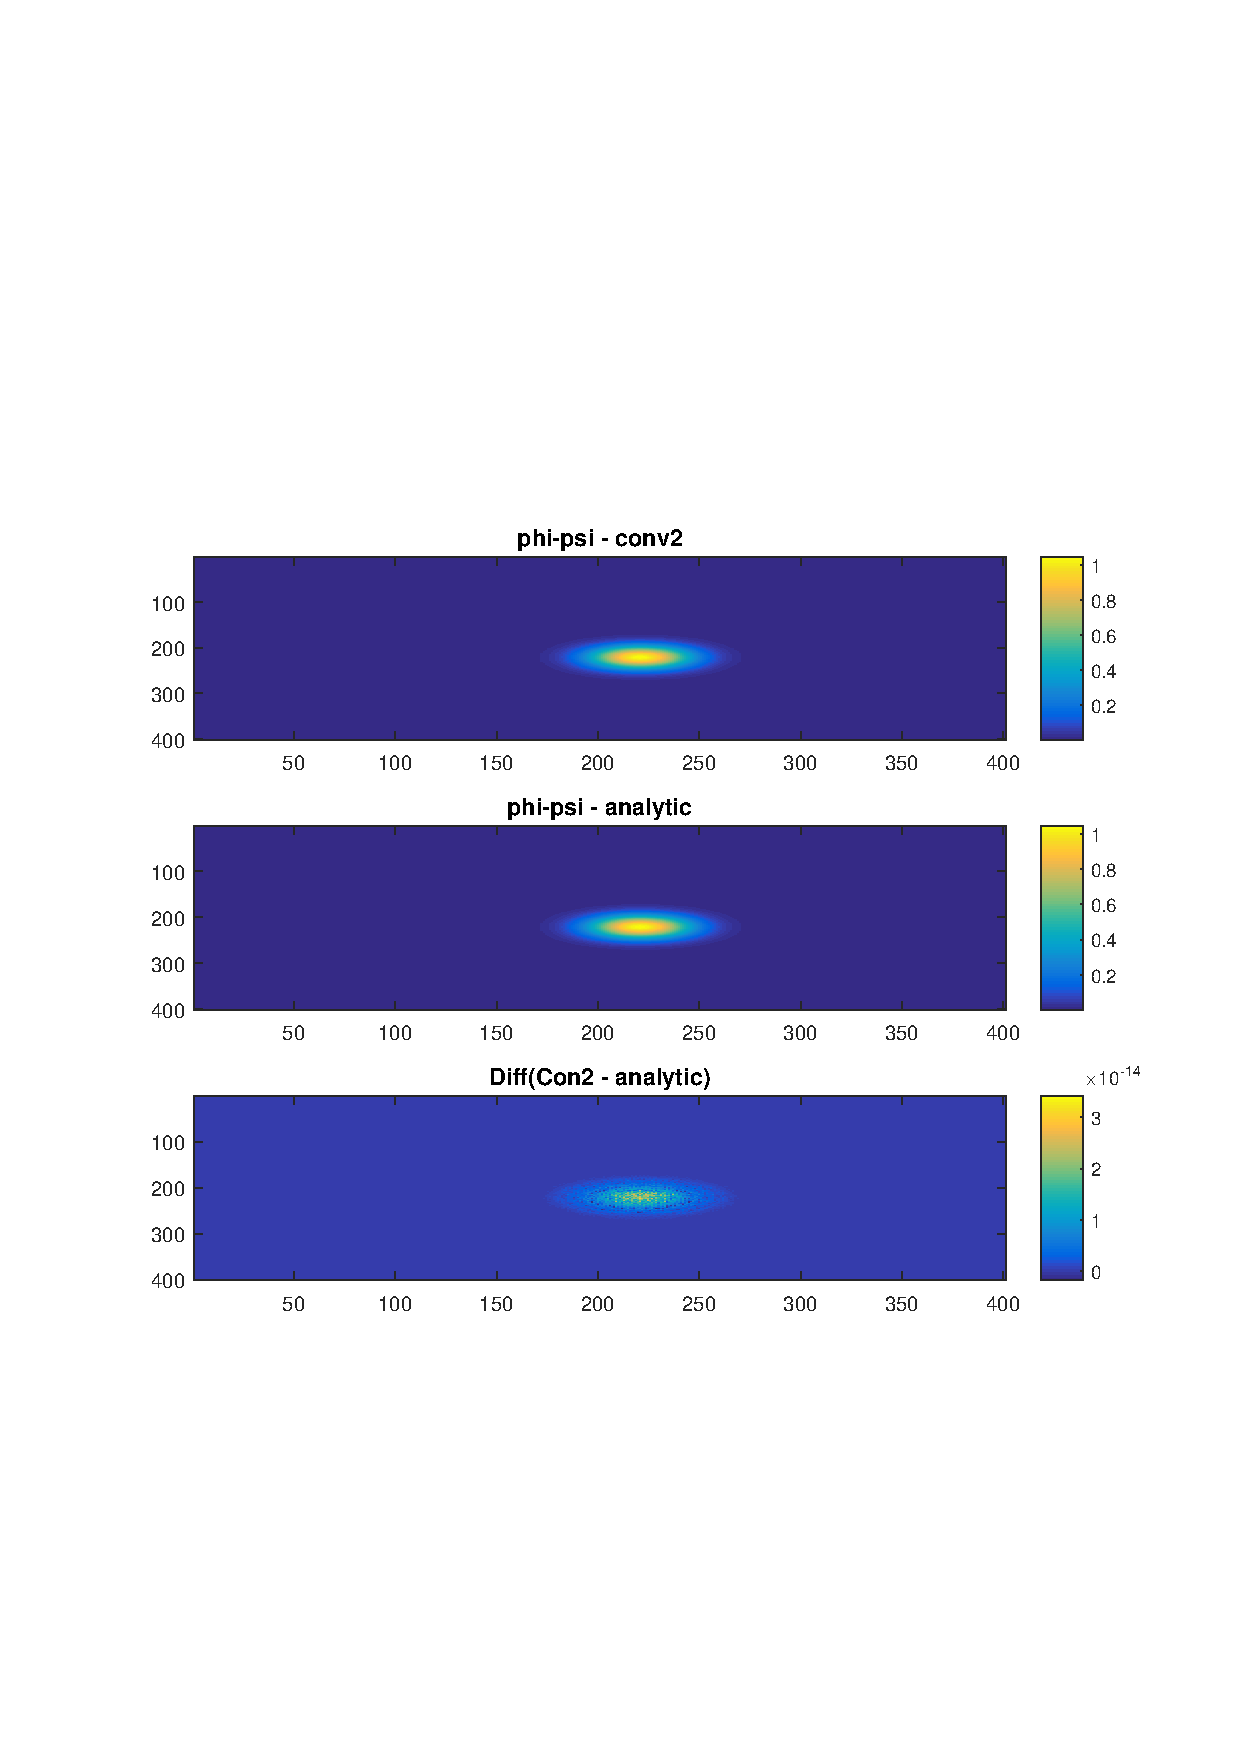
\includegraphics[width=\textwidth]{Convolution2DGaussians_Analytic_Conv2.pdf}
\caption{Residual(analytic, Conv2)}\label{Convolution2DGaussians_Analytic_Conv2.pdf}
\end{figure}



\newpage




% Compute Gamma
\section{Compute Gamma}

\paragraph{We analytically estimate Gamma matrix based on Equation (21) and Equation
(D.7) in Appendix D.}

\paragraph{We decompose neural field into a finite-dimentional state vector. Each element
of the state vector is a Gaussian basis function.}

\paragraph{Define $\Gamma=\int_{\Omega}\phi(r)\phi^{T}(r)dr$. Firstly, programmatically
define $\phi(r)$, as a vector of Gaussian basis functions. Each Gaussian
function is defined as $\phi(r-r')=\exp{(-\frac{(r-r')^{T}(r-r')}{\sigma_{\phi}^{2}})}$.}

\paragraph{File (Matlab script): ComputeGamma.m}

\subsection{Parameter List}
\textbf{\textit{Input parameter list:}}\newline
SpaceMin - Edge of surface on the negative side\newline
SpaceMax - Edge of surface on the positive side\newline
NPoints - number of points along each dimension\newline
nx - number of Gaussian basis functions\newline
mu - centres of Gaussians, a 2 times Nx matrix\newline
sigma - variance-covariance matrix of each Gaussian\newline
\textbf{\textit{Output parameter list:}}\newline
gamma - gamma matrix

\subsection{Implementations}
\paragraph{Inner product of two Gaussians\newline}



\subsection{Results}
\begin{figure}[H]
\centering
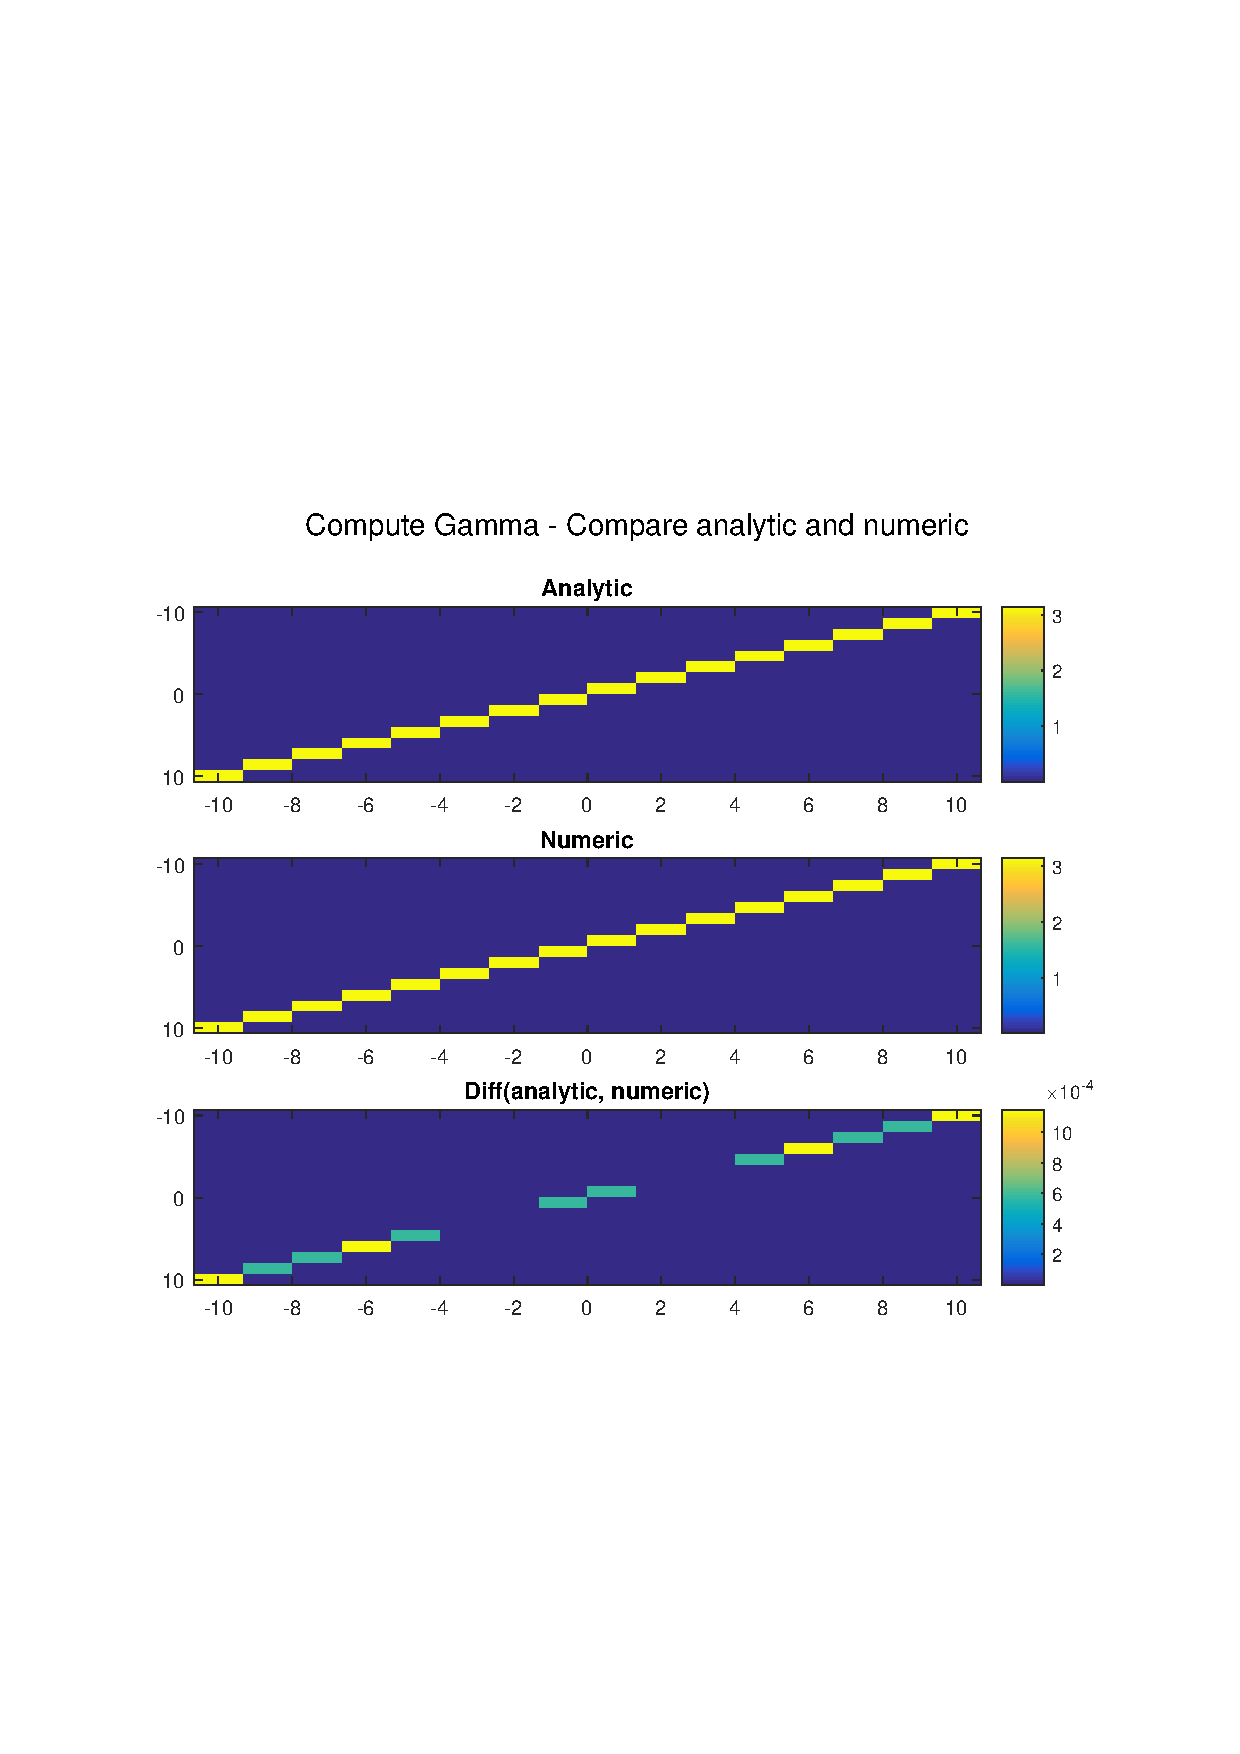
\includegraphics[width=\textwidth]{ComputeGamma_Check_AnalyticNumeric_SpatialRes_501.pdf}
\caption{Compare analytic and numeric results of computing Gamma}
\end{figure}

\newpage



% Compute Psi
\section{Compute Psi}
\paragraph{We will compute Psi Matrix, according to Equation (24). In this section, we
wiil use the Gamma matrix computed from the previous section.}
\paragraph{File (Matlab script): ComputePsi.m}


\subsection{Parameter List}
\textbf{\textit{Input parameters}:}\newline
SpaceMin - Edge of surface on the negative side \newline
SpaceMax - Edge of surface on the positive side \newline
NPoints - number of points along each dimension \newline
nTheta - number of connectivity kernel basis functions \newline
Ts - Time step \newline
nx - number of Gaussian basis functions \newline
mu\_phi - centre of Gaussian basis function for phi \newline
sigma\_phi - sigma of Gaussian basis function for phi \newline
mu\_psi - a vector of centres of Gaussian basis functions of connectivity kernel \newline
vector\_Sigma\_Psi - a vector of sigma of Gaussian basis functions \newline
\textbf{\textit{Output parameters}}:\newline
Psi - Psi matrix



\subsection{Implementations}

\paragraph{Pre-define parameters and centres of field basis functions\newline}
Define the coordinates of discretisation of the cortical surface as varialbe \textit{x}. If the centres of field basis function are left as empy the input parameters (mu\_phi, a
vectore of 2-D coordinates of centres), we define these centres here and spread them
uniformly in the cortical surface. \newline
We calculate the number of rows, \textit{numRow}, and columns, \textit{numCol}, based on the
number of field basis function, \textit{nx}.\newline
We align the centres of field basis functions to either right on the
discretisation points or the middle point of two adjacent discretisation
points, to avode introducing unnecessary dynamics. \newline
So, we have centres, \textit{mu\_phi}, and variance-covariance matrix, \textit{covMat\_phi},
of each field basis functions.\newline
\paragraph{Compute Gamma\newline}
Call function, \textit{ComputeGamma.m}, to compute Gamma matrix, \textit{Gamma} (a \(\textit{nx}\times
\textit{nx}\) matrix).\newline

\paragraph{Compute coefficients of convolution of phi and psi\newline}
A vector of Gaussian coefficients, \textit{psi\_phi\_coefficient} (\(1\times\textit{nTheta}\) vector), is computed based on Equation
(E.4) Appendix E.

\paragraph{Compute convolution of phi and psi\newline}
To compute convolution of psi and phi analytically, we use function \textit{Define2DGaussian\_AnisotropicKernel.m}
to define Gaussian basis and times the coefficients, \textit{psi\_phi\_coefficient}.
The resultant Gaussians are stored in variable \textit{psi\_phi\_basis}

\paragraph{Compute Psi matrix\newline}
Firstly we inverse Gamma matrix as \textit{inv\_Gamma}. Then we times time step, \textit{Ts} (constant), and \textit{inv\_Gamma} to each row of \textit{psi\_phi\_basis}.
The result is Psi matrix and it's stored in variable \textit{Ts\_invGamma\_phi\_psi} and is returned back to the function.

\subsection{Results}
Run script: ComputePsi\_Compare\_AnalyticNumeric.m
\begin{figure}[H]
\centering
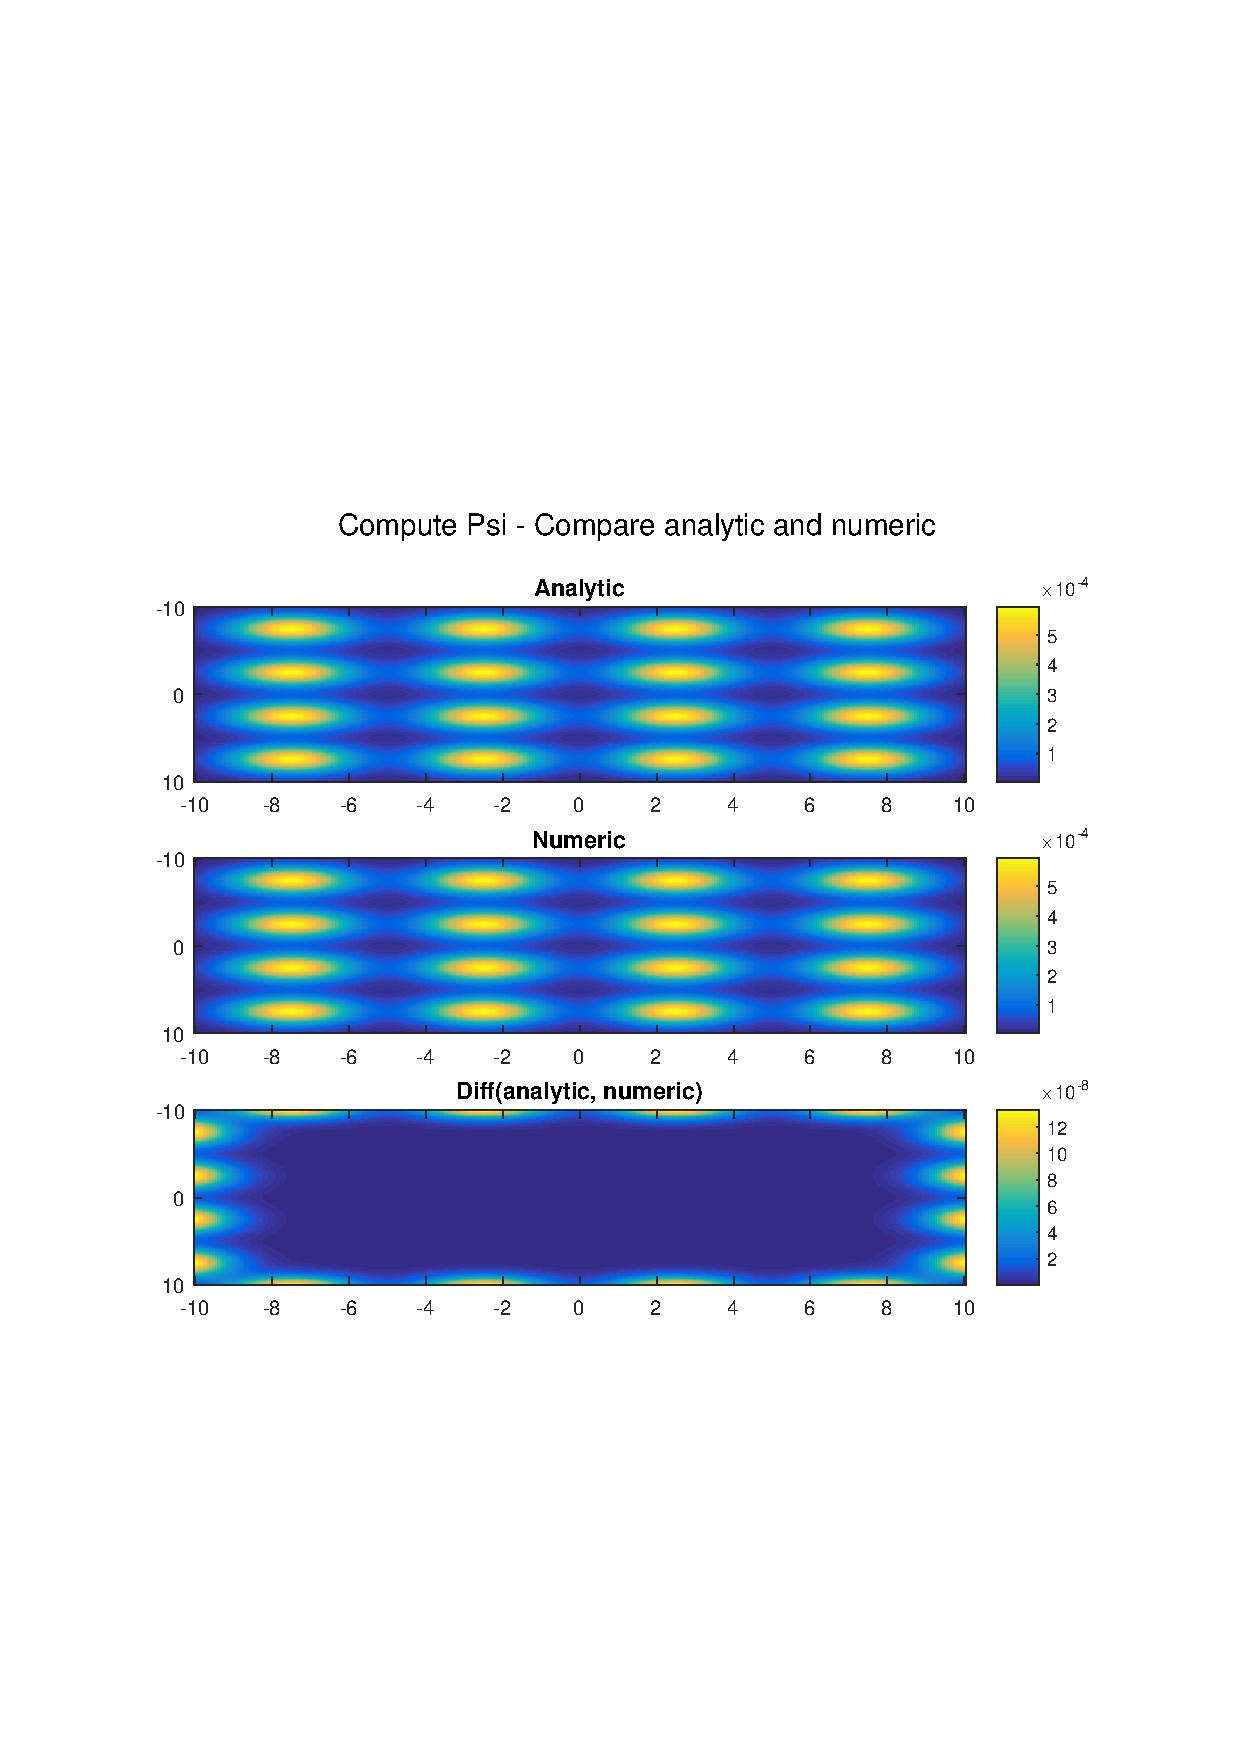
\includegraphics[width=\textwidth]{ComputePsi_Check_AnalyticNumeric_SpatialRes_301.pdf}
\caption{Compare analytic and numeric results of computing Psi}
\end{figure}
\newpage


\section{Compute State Vector at time T+1}
\label{state vector}
\paragraph{parameter table, figures}
\subsection{Parameter List}
\subsection{Implementations}
\subsection{Results}
\newpage





\section{Compute Reduced Model}
\subsection{Parameter List}
\subsection{Implementations}
\subsection{Results}

\newpage





\section{Compute Full Model}
\paragraph{We numerically compute neural field at time T+1 based on field at time T.
As opposed to reduced model, full model does not decompose neural field into field basis functions; it directly convolves
the neural field at time T with connectivity kernel.}

\subparagraph{In the full model, when we convolve neural field at time T with connectivity kernel,
we have significant errors or residual on the edges of the field. In order to conquer this,
we apply a boundary condition method to extend the field into 9 tiles and each tile is an identical copy
of the neural field.}

\subsection{Parameters}
\subsection{Implementations}
\subsection{Results}
\newpage


\section{Compare Reduced Model and Full Model}
\paragraph{Compare neural fields at time T+1 computed by reduced model and full model.\newline
Script name: Compare\_CompleteModel\_ReducedModel.m}
\subsection{Parameters}
\subsection{Implementations}
\subsection{Results}


\begin{figure}[H]
\centering
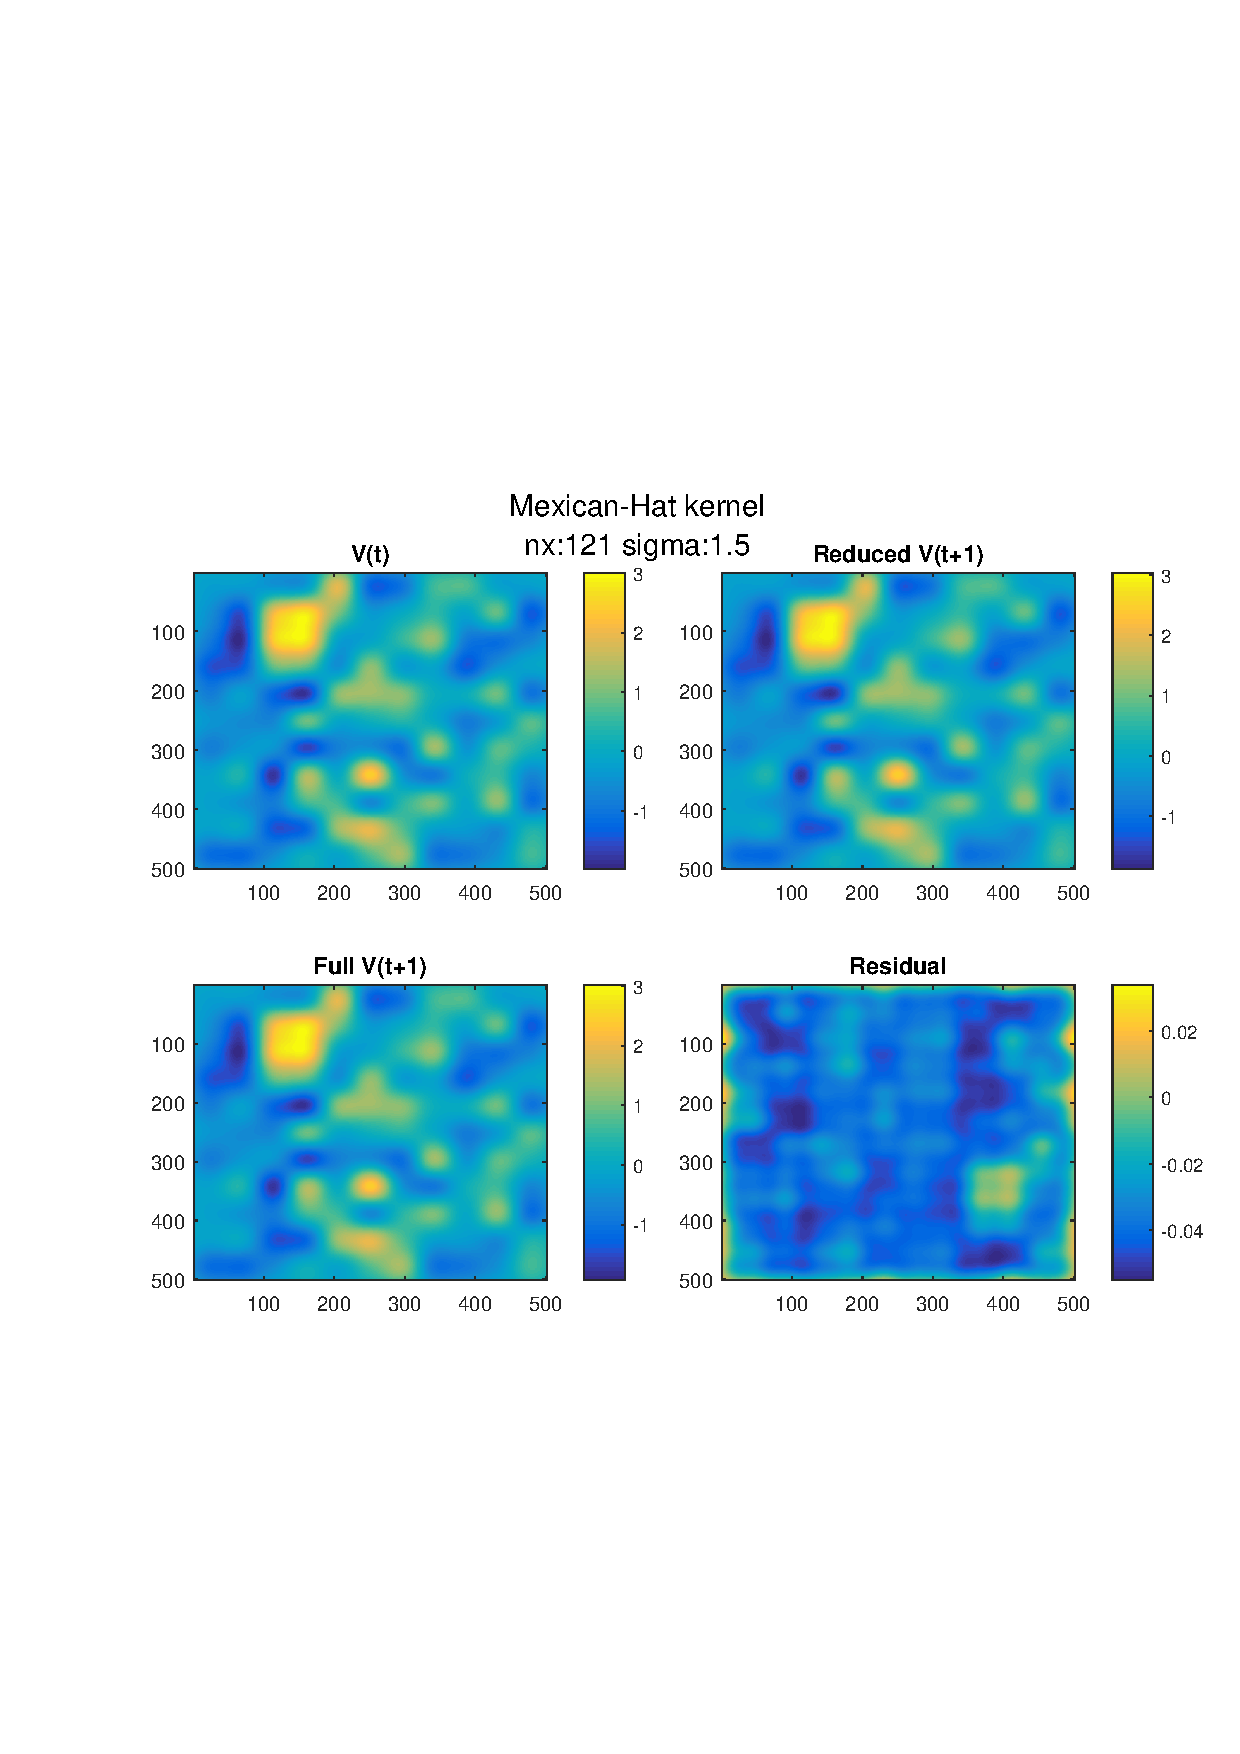
\includegraphics[width=\textwidth]{modelComparison_MexHat_nx_121_sigma_1_5_nPoints_501_vTPlus1.pdf}
\caption{Connectivity kernel, Mexican Hat}
\end{figure}


\end{document}
